\section{General-purpose input/output (GPIO)}

%----------------------------------------------------------------------------------------
%	DEFINITION SUBSECTION
%----------------------------------------------------------------------------------------

\subsection{Definition}
General-purpose input/output (GPIO) is a generic pin on an integrated circuit or computer board whose behavior including whether it is an input or output pin is controllable by the user at run time.

GPIO pins have no predefined purpose, and go unused by default. The idea is that sometimes a system integrator who is building a full system might need a handful of additional digital control lines and having these available from a chip avoids having to arrange additional circuitry to provide them. For example, the Realtek ALC260 chips (audio codec) have 8 GPIO pins, which go unused by default.

%----------------------------------------------------------------------------------------
%	Atmega32 GPIO SUBSECTION
%----------------------------------------------------------------------------------------

\subsection{Atmega32 GPIO}
Atmega32 has 8-bit port, i.e. it has 8 pins in a single port. Each bit represents a pin i.e. bit 0 represents pin 0 on that port and so on. As you can see in the diagram given below, Atmega32 has 4 ports named as A, B, C \& D. Each of these ports has 8-pins (micro-controller pins).\\

\centerline{
	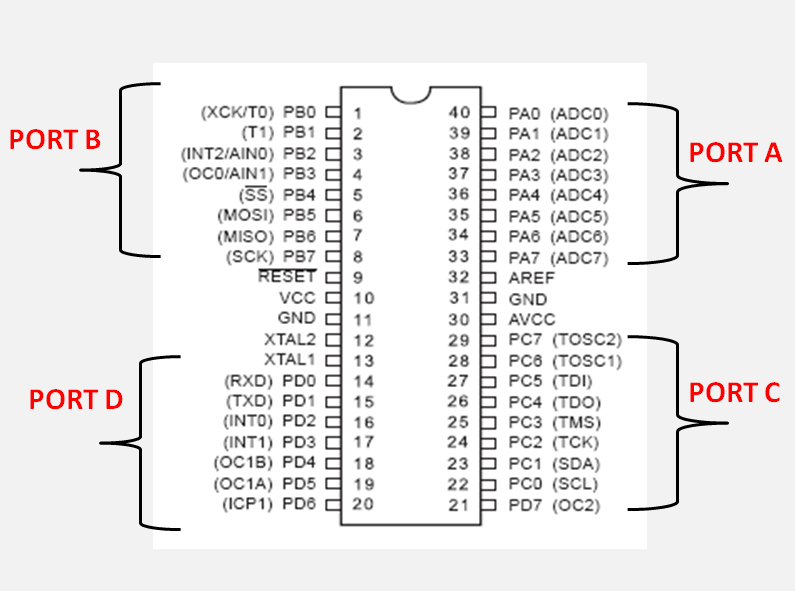
\includegraphics[width=0.8\textwidth]{overview/images/gpio.png}
}

%----------------------------------------------------------------------------------------
%	GPIO REGISTERS SUBSECTION
%----------------------------------------------------------------------------------------

\subsection{GPIO REGISTERS}
Every GPIO has three registers associated with it in order to control a particular pin. For AVR micro-controllers these registers are:

\begin{enumerate}
  \item DDRn – Data Direction Register
  \item PORTn – Port Output data Register
  \item PINn – Port Input Register
\end{enumerate}

\textbf{n} - Indicates the port name i.e. A, B, C \& D 
\\

\centerline{
	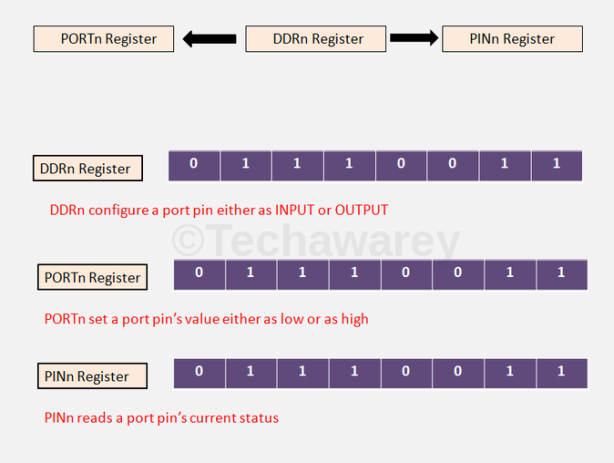
\includegraphics[width=0.8\textwidth]{overview/images/gpio-registers.png}
}

%----------------------------------------------------------------------------------------
%	DDRn REGISTERS SUBSECTION
%----------------------------------------------------------------------------------------

\subsubsection{DDRn Register}
Data Direction Register configures data direction of a port or a port pin. I mean a port will used for input or output.
\\\\
Writing a value 0 configure that port pin as INPUT and writing a value 1 configures a port pin as OUTPUT.

%----------------------------------------------------------------------------------------
%	PORTn REGISTERS SUBSECTION
%----------------------------------------------------------------------------------------

\subsubsection{PORTn Register}
PORTn register is used for two purposes : \\
\begin{enumerate}
	\item To output data when port is configured as output
    \item To activate/deactivate internal pull-up registers when port is configures as input
\end{enumerate}

%----------------------------------------------------------------------------------------
%	PIN REGISTERS SUBSECTION
%----------------------------------------------------------------------------------------

\subsubsection{PIN Register}
The PINn register keeps the status of all the pins in that port. By reading this register we can get the current logic level (0 or 1) on the pin. When the pin is configured as input, this register tells what logic level is being given on that pin, whether it’s 0 or 1. When the pin is configured as output, this register tells what logic level is being driven out.111

%----------------------------------------------------------------------------------------
